\chapter{Freebusy}
\label{Freebusy}
Freebusy Informationen des pers�nlichen LV-Plans eines Users stehen unter foglender URL zur Verf�gung:
\\
https://cis.technikum-wien.at/cis/public/freebusy.php/<username>\\
\\
<username> ist durch den Loginnamen zu ersetzten.\\
\\
Die Freebusy URL enth�lt standardm��ig den pers�nlichen LV-Plan des Users.
Es gibt die M�glichkeit, diese Freebusy URL zu erweitern, um pers�nliche Kalender in diese URL mitaufzunehmen. (zB Horde Webmail, Google Kalender, DAViCal, etc)
\section{Zus�tzliche Freebusy URLs hinzuf�gen}
�ber den Punkt ''Neuen Eintrag hinzuf�gen'' k�nnen zus�tzliche Freebusy URLs hinzugef�gt werden.
Alle Eintr�ge werden zu einer gesammelten Freebusy URL vereint.

\begin{figure}[ht]
\begin{center}
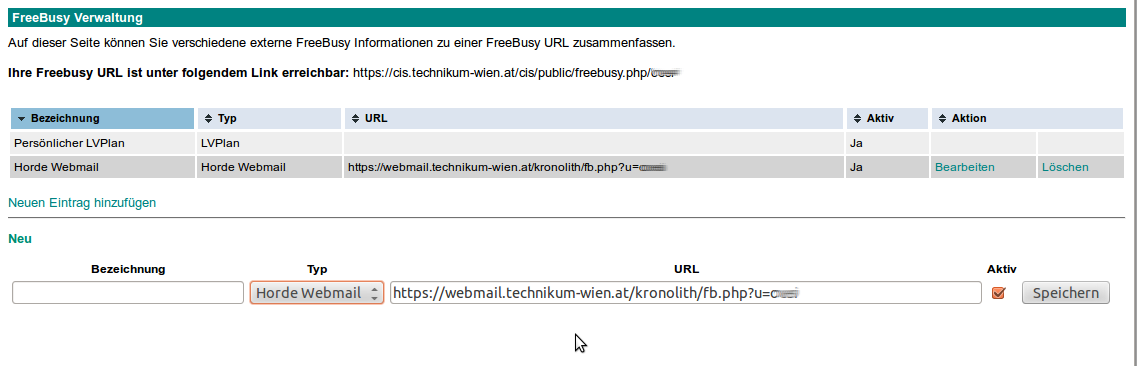
\includegraphics[width=1.0\textwidth]{freebusy_neu.png}
\end{center}
\caption{FreeBusy URL hinzuf�gen}\label{FreeBusy URL hinzuf�gen}
\end{figure}

\begin{enumerate}
	\item Bezeichnung: Freitext Bezeichnung der URL
	\item Typ: Anbieter der URL
	\item URL: Pfad zur FreeBusy URL die hinzugef�gt werden soll (wird in manchen F�llen bei der Auswahl des Typs vorgeschlagen)
	\item Aktiv: Dieses Hackerl muss gesetzt sein, damit die Eintr�ge in die FreeBusy URL aufgenommen werden
\end{enumerate}

Der pers�nliche LVPlan ist automatisch zur FreeBusy URL zugeordnet und kann nicht entfernt werden.